\label{classification}
A part of this thesis was the categorization of the scraped pages. Categorization in this context means the procedure of assigning categories (labels) to pages. The data set at hand contained a vast amount of pages, as we discussed in Chapter \ref{datasetAnalysis}. The manual categorization of this number of pages would therefore take too much time and in consequence was infeasible. An automatic system for text classification was required. A simple system with a list of words assigned to each label (naive approach) was introduced but was performing poorly. The naive approach is outlined in Section \ref{naiveApproach}. A more sophisticated tool for text categorization is machine learning. We decided to use supervised machine learning (ML).

This chapter describes the naive approach. Secondly ML in general is characterized. Then, the main approaches of ML, reinforcement learning(RLr), unsupervised learning (ULr), and supervised learning (SLr), are characterized. Lastly we depict what an artificial neural network (ANN) is. The approach used in this thesis is a type of an ANN using SLr.


 \section{Naive approach} \label{naiveApproach}
The naive approach first leveraged for the classification on a sample of about 4,000 pages was a two dimensional (2D) list\footnote{With 2D list we mean a list of lists.} with words. The first dimension represented the categories. The second dimension was a list filled with words frequently associated with the category the list was dedicated to. For example the list for the category \textit{Drugs} contained among others the words \textit{weed, marihuana, cannabis, cocaine, coke, hashish, heroine, grams, drugs, ecstasy}. Such a list was created for each category. The categories will be described in more detail in Chapter \ref{classificationCategories}. Next, the words in the content of the pages were normalized and the twenty most frequent words of each page were compared to the 2D list. Each conformity was counted and the results were stored in a list as a category - conformity-count pair. The category with the highest conformity-count was then assigned to the page. The accuracy of this approach was below 40\%.

The 2D list was not exhaustive. In order to include all the relevant words for every category we would need to study the data set extensively. This in unviable in the context of the data load as we discussed earlier in this chapter. Also, special meanings of specific words would not be taken into consideration. For example the words \textit{red room} have a special meaning. This naive approach could not detect such connections. In light of the listed problems we decided to not pursue this technique further.


\section{Machine learning} \label{machineLearning}
The term \textit{machine learning} was first introduced by Arthur Samuel. In his paper \textit{Some Studies in Machine Learning Using the Game of Checkers} \cite{machineLearningOriginal} he proved it is possible for a program to develop better game-related skills than the skills of the programmer of the program.

ML is the procedure in which an agent\footnote{A system utilizing ML to learn and adapt autonomously \cite{machineLeraningApproaches}} creates a model which develops the ability to perform a certain task. The learning process is based on the evaluation of gained experience \cite{machineLearningToday}. The agent requires an initial data set in order to train and validate. The size of the initial data set depends on the nature of the task and the selected ML type and set of algorithms. During training the agent attempts to perform the given task and validates its own performance. The agent then adjusts its criteria for performing the task based on the validation results. These two steps are repeated a number of times defined by the programmer. The output of the agent is a model able to perform the task it was trained for. 

ML is used across various industries and fields. The need for automated analysis is increasing with the growing popularity of \textit{big data}\footnote{A data set too vast or complex for traditional or manual data processing.} \cite{bigDataExplained} \cite{bigDataPopularity}. ML is used widely with Big Data. ML is also used in the language processing field \cite{machineLearningToday}. Examples include virtual assistants or instant translation tools. Another use for ML is in the automotive industry. Cars with assisted parking or breaking, or self-driving cars are examples\cite{selfDrivingCars}. Also, ML is used frequently in games for a more natural game experience \cite{machineLearningGaming}. 

There are several approaches in ML based on the different ways of training. We describe the three main approaches in the subsections following. Namely \textit{reinforcement learning} in Subsection \ref{reinforcementLearning}, \textit{unsupervised learning} in Subsection \ref{unsupervisedLearning}, and \textit{supervised learning} in Subsection \ref{supervisedLearning}. The approach used in this thesis was \textit{supervised learning}. 

\subsection{Reinforcement learning} \label{reinforcementLearning}
It is suitable to use RLr if behaviours in dynamic environments are to be learned \cite{reinforcementLearningIntroduction}. A software agent receives an indication of the state of the environment. The agent then pics an action from a discrete set of agent actions. Next the state is modified by the action. The value of this modification is passed on as a scalar reinforcement signal to the agent. The objective for the agent is to maximize the long-run total of reinforcement signal values. This is achieved over time by leveraging a number of specialized algorithms together with methodical trial and error. RLr is well suited for example for the development of game-behaviour \cite{reinforcementLearningGames}.

\subsection{Unsupervised learning} \label{unsupervisedLearning}
 ULr is used when seeking common patterns or relationships in data. It is also commonly used when trying to find anomalies in data \cite{unsupervisedLearningIntroduction}. The software agent receives an unlabeled data set as input. The agent breaks the data down to critical components using specialized algorithms. It then identifies similarities and divides the data into groups. No feedback is involved. One of the fields ULr is used is astronomy. For example for tasks such as estimating the photometric  redshifts or finding galaxy clusters \cite{unsuperviseLEarningAstronomy}. 

\subsection{Supervised learning} \label{supervisedLearning}
SLr is suitable to use for the classification of data. During training SLr relies on labeled data \cite{machineLeraningApproaches}. The input of the software agent of SLr is a labeled data set. The software agent divides the data---label pairs into a training and test set randomly. The agent is to find a function with the data as input and the correct label as output. To achieve this the agent is trained on the training set and validated using the test set. After each run the accuracy and loss is computed and the function is modified with the goal to improve the future output. SLr is suited for example for the classification of data \cite{supervisedLearningClassification}. 

\section{Artificial neural networks} \label{artificialNeuralNetworks}
An ANN is a ML system inspired by animal brains \cite{machineLeraningApproaches}. A brain is composed of components such as neurons. Neurons communicate with each other by passing information through synapses. The more often two neurons communicate the stronger the synapses between them are \cite{neuronsInBrain}. This results in a neuron prioritizing information passed by neurons participating in frequent communication. 

A structure of an ANN is portrayed in Figure \ref{structureOfCNN}. An ANN is comprised of layers of nodes sometimes also called \textit{neurons}. The neurons communicate via directed links of various relevance also called \textit{weight}. The weight is represented by a real number. A neuron determines whether to react to information gathered through a link according to its weight passed to an \textit{activation function}. We discuss activation functions later in Subsection (AcF) \ref{activationFunction}. Neurons exist in groups called \textit{layers}. Layers used in this thesis were \textit{embedding layers} \ref{embeddingLayers}, \textit{convolutional layers} \ref{convolutionalLayers}, \textit{polling layers} \ref{poolingLayers}, and \textit{dense layers} \ref{denseLayers}. All of the used layers are described closer in the next subsections. Layers between the input and output layers are called \textit{hidden layers}. If an ANN contains convolutional layers it is called a convolutional neural network (CNN).
\begin{figure}[ht!]
  \centering
  \includegraphics[width=\textwidth]{Images/structureOfCNN.png}
  \caption{An illustration of the CNN implemented in this thesis. The two portrayed dense layers are a modified image from an article on deep learning \cite{structureOfCNN}. The individual layers are detailed in Section \ref{artificialNeuralNetworks}.} 
  \label{structureOfCNN}
\end{figure} 

One learning cycle is called an \textit{epoch}. In case of big data sets the data are divided into smaller chunks of data. These chunks are called \textit{mini-batches}. In this paragraph we characterize a typical cycle over a mini-batches (batch-cycle) in an ANN using SLr. A single epoch consists of at least one batch-cycle. At the beginning of a batch-cycle the training data are passed to the first layer. Data are passed from one layer to the next one. Every layer modifies the received data before passing it on. The manner in which the data are modified depends on the type of the layer. After the data are processed by the last layer the output model is evaluated using the testing data. Improving the model is now the objective. A way leveraged to improve accuracy is first the calculation of the loss by utilizing a \textit{loss function}. The loss function is outlined in more detail in Subsection \ref{lossFunction}. After evaluating the loss the weights of the neurons are adjusted by the \textit{backward propagation of errors} detailed in Subsection \ref{backpropagation}. After the weights of the first layer have been adjusted the batch-cycle ends. The epoch ends after all batch-cycles finish. The number of batch-cycles in an epoch depends on the number of mini-batches. The number of batch-cycles and epochs is specified by the programmer. 

\subsection{Embedding layer}\label{embeddingLayers}
Embeddings \cite{embeddingsOverview} compose a matrix of word aliases representing how semantically meaningful relations between words are. For example the relation between the words \textit{queen} and \textit{princess} is in some way similar to the relation between the words \textit{mother} and \textit{daughter}. An ANN operating on words achieves good results if some sort of embedding is adopted \cite{goodToUseEmbeddings}. An embedding layer (EmbLr) creates an embedding matrix via training. The matrix is generated by assigning embedding vectors to each word in a vocabulary of all words in the input. The distance between the vectors of two words describes the relations between them. From the vectors of the previous example the result vector could imply $queen - princess = is~predecessor~of$. 

The EmbLr may also use a pre-trained embedding matrix. The layer then passes the input words replaced by the embedding vectors to the next layer. 

\subsection{Convolutional layer}\label{convolutionalLayers}
Convolutional layers (ConvL) are suited for finding features in data~\cite{CNN}. A ConvL decreases the~ size and complexity of~the~input by convoluting the input. The convolution of data are a way of combining two sets of data.  It does so by sliding a \textit{filter}, also called kernel, of a certain size with a certain stride across the input and performing a \textit{convolution operation} (ConvO). An example of a simple ConvO is visualized in figure~\ref{convolutionalLayerVisualization}. The stride size represents the number of input-units, e.g. pixels, the kernel needs to skip in order to perform the next ConvO\footnote{The sliding direction is to the right. If sliding to the right is not possible the filter is returned to the very left and stride-size down. If sliding down is not viable the sliding is finished.}. The kernel is represented by real numbers and is initialized with random numbers. A ConvO can have multiple kernels. Each kernel is applied to a portion of the image corresponding to the kernel size, called the \textit{receptive field}~\cite{receptiveField}. This action is called a (ConvO). After applying the kernel to all possible receptive fields the output of the layer is generally smaller in size than the input. It is, however, possible for the output dimensions to be the same as the input dimensions. Moreover, the information carried in the borders of the input may not be lost. This is useful when the number of ConcLs is rather sizable. It is achieved by applying \textit{padding}. Padding is the practice of adding information around the borders of the input, e.g. \textit{zero-padding}\footnote{Zero-padding is a specific type of padding. The input is enriched with zeros around the borders.}. The result of the convolution is fed to a specified AcF. AcF is detailed in the later Subsection \ref{activationFunction}.
\begin{figure}[ht!]
  \centering
  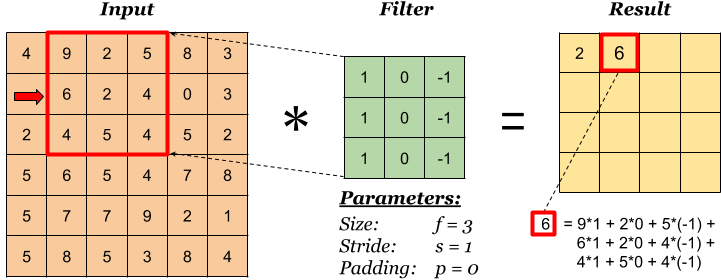
\includegraphics[width=\textwidth]{Images/convolutionOperation.png}
  \caption{The visualized process of a ConvO \cite{convolutionOperationVisualization}. The very left square is the input -- a 2D image of size 6x6 pixels. The square in the center depicts a 3x3 kernel with no padding. The stride of the kernel is 1 pixel. The very right square represents the partial result after the kernel was applied to two sections of the input. The final output will be of size 4x4 pixels. The ConvO itself is enumerated under the output image.} 
  \label{convolutionalLayerVisualization}
\end{figure} 

The first ConvL implemented in this thesis receives as its input the normalized and encoded content of the scraped pages. The other ConvLs receive their input modified by other layers. The ConvLs then proceed as described earlier. In doing so the size of the output compared to the input is reduced. Also, features of the input significant to the layer are highlighted. 

\subsection{Pooling layer}\label{poolingLayers}
Pooling layers (PoolL) reduce the size of the input by down-sampling. The procedure resembles a sliding window of a certain size sliding over the input with a certain stride. The stride in this layer is similar to the stride in ConvLs \ref{convolutionalLayers}. The result of each step of the pooling depends on the method used. There are several types of methods to choose from for the PooL. One of the most used type is \textit{max-pooling} \cite{CNN}. The result of max-pooling is the maximum value from the values currently present in the filter window. After applying the filter to all input portions the result is passed to the next layer.
\begin{figure}[ht!]
  \centering
  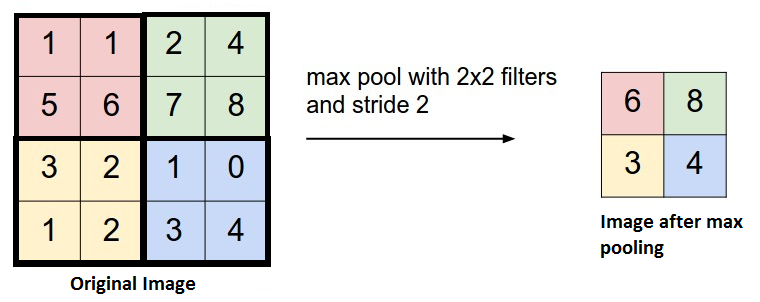
\includegraphics[width=\textwidth]{Images/maxPooling.png}
  \caption{The visualized process of max-pooling with filter size of 2x2 pixels and stride length of 2 pixels by Analytics Vidhya~\cite{maxPoolingVisualization}. The input is a 2D image and is depicted by a square with scalar values. The size of the image is 4x4 pixels. The square on the right is the result after max-pooling is applied on the input. The output image is of size 2x2 pixels. The max-pooling process is described in Subsection \ref{poolingLayers}.} 
  \label{maxPoolingVisualization}
\end{figure} 

A simple example case of max-pooling is shown in Figure \ref{maxPoolingVisualization}. In the beginning the upper left corner of the filter is set to be in the upper left corner of the input which is the red part of the image. The maximum value from the values \textit{1; 1; 5; 6;} is \textit{6}. The filter therefore returns the red result \textit{6}. Next the upper left corner of the filter moves two pixels to the right. It now occupies the green part of the input image. It again performs the max-pooling operation. It is not possible for the filter to slide right anymore as the end of the input was reached. The filter is therefore returned to the beginning of the line and moved two pixels down into the yellow portion. After returning the yellow result the filter slides two pixels to the right and once more return the maximum value. It is not possible to move the filter right nor down. The Max-pooling now is finished an the result is the square on the right.

The PoolLs implemented in this thesis receive as their input the output of the foregoing ConvL. The layer applies max-pooling. In doing so the size of the next input is again reduced by selecting the maximum features.

\subsection{Dense layer}\label{denseLayers}
Each neuron in a dense layer (DnsL) is directly connected to all the neurons from the previous layer as well as to all neurons in the next layer \cite{CNN}. DnsLs are therefore also called fully connected layers. DnsLs are well suited for classification tasks. A DnsL is visualized in figure~\ref{denseLayerVisualization}. The advantage of a DnsL is every output of every neuron of the previous layer is processed. The outcome ${z^l_n}$ for neuron ${n^l}$  is enumerated as a multiplication of two matrices \textit{w} and \textit{x} with the formula \[{z^l_{n}}=w^l_n  x^l + b^l_n~\cite{neuronFormula}\text{.}\] Where ${n^l}$ is a node belonging to layer ${l}$. Weight ${w^l_n}$ are all weights of direct connections into neuron ${n^l}$ and \textit{x} are all inputs of said connections into neuron ${n^l}$. The notation ${b^l_n}$ symbolizes the bias of node ${n^l}$. The result of the operation described is fed to a specified AcF. AcF is detailed in Subsection \ref{activationFunction}. The main disadvantage of DnsLs is the number of input arguments.
\begin{SCfigure}
  \includegraphics[width=0.5\textwidth]{Images/denseLayer.png}
  \caption[rightcaption]{The visible portion of this network consists of a DnsL ${l^1}$. This layer is composed of two neurons, ${n^1_0}$ and ${n^1_1}$ and their corresponding biases ${b^1_0}$ and ${b^1_1}$. Each neuron receives two inputs ${x^1_{0}}$ and ${x^1_{1}}$ with weights ${w^1_{00}}$, ${w^1_{01}}$, ${w^1_{10}}$, and ${w^1_{11}}$ respectively. The operation the neurons of the DnsL perform is now described on neuron ${n^1_{0}}$. Neuron ${n^1_{0}}$ computes the outcome ${z^1_{00}}$ as 
${w^1_{n}}$~$\cdot$~${x^1}$~+~${b^1_0}$~=~
 $\left(\begin{smallmatrix}{w^1_{00}}&{w^1_{01}}\end{smallmatrix}\right)$$\cdot$$\left(\begin{smallmatrix}{x^1_{0}}\\{x^1_{1}}\end{smallmatrix}\right)$~+~${b^1_0}$
which is broken down to ${w^1_{00}}$~$\cdot$~${x^1_{0}}$~+~${w^1_{01}}$~$\cdot$~${x^1_{1}}$~+~${b^1_0}$.
}
  \label{denseLayerVisualization}
\end{SCfigure} 

The first DnsL implemented in this thesis receives as its input the output of the last pooling layer. It then proceeds as described earlier. The second DnsL receives its input from the first DnsL. This layer ensures the classification of the data.

\subsection{Activation function}\label{activationFunction}
An activation function (AcF) is used to modify the output of a neuron most commonly in a non-linear way in order to limit the amplitude of the output of a neuron \cite{activationFunction}. The output of an activation function is called \textit{unit's activation} or just \text{activation}. There are many types of AcFs. In this thesis we used the AcF called \textit{rectified linear unit} (ReLU) and \textit{softmax}.

\textbf{ReLU} is an AcF used in multilayer networks \cite{ReLU}. The function itself is shown in Figure \ref{reluImage}. It is expressed as 
\[\sigma(x)= \begin{cases}
    0, & \text{for } x\leq 0\\
    x, & \text{for } x > 0
\end{cases}~\cite{ReLU}\] ~where $\sigma$ represents ReLU. ReLU is used for its reduction of activation since only positive input values are having a non-zero output. Another advantage is information of positive input values is not lost.
\begin{figure}[ht!]
  \centering
  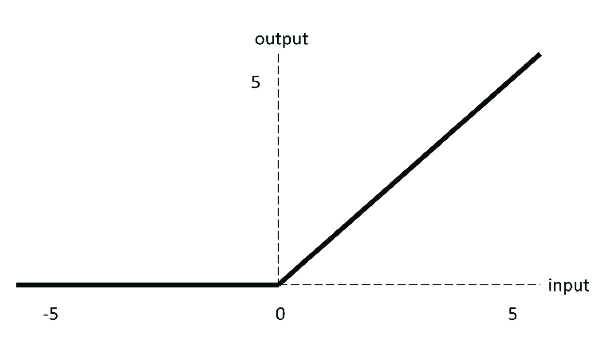
\includegraphics[width=0.8\textwidth]{Images/ReLUFunction.png}
  \caption{The ReLU AcF from the Multi-classification of Brain Tumor Images using Deep Neural Network \cite{reluImage} article.} 
  \label{reluImage}
\end{figure} 

\textbf{Softmax} is an AcF leveraged for the designation of probabilities of an input belonging to beforehand given labels \cite{machineLeraningApproaches}. The activation is a vector of numbers each between 0 and 1. Each number represents the probability of the input belonging to the current label.  In our case labels were categories of pages.

\subsection{Loss function}\label{lossFunction}]
As was discussed in Section \ref{artificialNeuralNetworks}, an ANN needs to learn in order to improve results. To be able to claim the results have improved an objective measure needs to be introduced. \textit{Utility} represents such a measure \cite{machineLeraningApproaches}. By utility we mean the total satisfaction of the learning agent. A way to obtain the amount of utilities lost is to utilize a loss function (LsF). Most generally, a LsF receives an input \textit{x}, the actual label of the input \textit{y} and the predicted label $\hat{y}$. The result of the LsF is computed as
\[
\begin{aligned}
LsF(x, y, \hat{y}) = Utility(\text{result of using }y \text{ given an input }x) \\
- Utility(\text{result using }\hat{y} \text{ given an input }x)~\cite{machineLeraningApproaches}
\end{aligned}
\]
There are several LsFs. The one we used is called \textit{categorical crossentropy} (CCross). 

\textbf{CCross} is used when the task is to label inputs and the amount of available labels is more than two \cite{categoricalCrossEntropy}. Also, it must be possible to assign each label with the likeliness of it belonging to the given input. The formula for CCross loss computation is
\[
-\sum\limits_{c=1}^M y_{i,c} log(p_{i, c})~\cite{categoricalCrossEntropy}
\]
where \textit{M} symbolizes the total number of labels and $c$ is the predicted label\footnote{Labels are represented by scalar values. Labels are converted if they were of non-scalar format, such as text.}.The symbol $y_{i, c}$ denotes a binary indicator\footnote{An indicator which holds one of two exclusive values, such as $0$ and $1$ .} signaling whether $c$ is the correct label for sample $i$. The symbol $p_{i, c}$ stands for the predicted probability that sample $i$ belongs to label $c$. 


\subsection{Backward propagation of error}\label{backpropagation}
The ouputs of individual layers need to improve in order to improve the results of an ANN. It is rather simple to determine the loss of the last layer utilizing the LsF. However, it is not possible to determine the loss of hidden layers in the same way. Therefore the error from the last layer needs to be propagated to the previous layers. This procedure is called backward propagation of error (back-prop) \cite{machineLeraningApproaches}. 

The weights and filters of individual layers are modified so that after the next forward-propagation\footnote{The flow of the data in the direction from the input layer to the output layer as opposed to backward-propagation.} the LsF output is smaller. The way the weights and filters are modified depends on various factors, e.g. the type of the layer, the AcF used, or the position the layer is in.

In case mini-batches are used back-prop alone is not efficient in minimizing the output of the LsF. Therefore optimizer algorithms are introduced into the back-prop. The goal of optimizers is to make the output of the LsF converge to the global minimum of the LsF in  a smaller number of epochs. The optimizer used in this thesis is RMSprop. RMSprop updates the weights dynamically based on the history of the weight values.